% Options for packages loaded elsewhere
\PassOptionsToPackage{unicode}{hyperref}
\PassOptionsToPackage{hyphens}{url}
\documentclass[
]{article}
\usepackage{xcolor}
\usepackage{amsmath,amssymb}
\setcounter{secnumdepth}{-\maxdimen} % remove section numbering
\usepackage{iftex}
\ifPDFTeX
  \usepackage[T1]{fontenc}
  \usepackage[utf8]{inputenc}
  \usepackage{textcomp} % provide euro and other symbols
\else % if luatex or xetex
  \usepackage{unicode-math} % this also loads fontspec
  \defaultfontfeatures{Scale=MatchLowercase}
  \defaultfontfeatures[\rmfamily]{Ligatures=TeX,Scale=1}
\fi
\usepackage{lmodern}
\ifPDFTeX\else
  % xetex/luatex font selection
\fi
% Use upquote if available, for straight quotes in verbatim environments
\IfFileExists{upquote.sty}{\usepackage{upquote}}{}
\IfFileExists{microtype.sty}{% use microtype if available
  \usepackage[]{microtype}
  \UseMicrotypeSet[protrusion]{basicmath} % disable protrusion for tt fonts
}{}
\makeatletter
\@ifundefined{KOMAClassName}{% if non-KOMA class
  \IfFileExists{parskip.sty}{%
    \usepackage{parskip}
  }{% else
    \setlength{\parindent}{0pt}
    \setlength{\parskip}{6pt plus 2pt minus 1pt}}
}{% if KOMA class
  \KOMAoptions{parskip=half}}
\makeatother
\usepackage{longtable,booktabs,array}
\newcounter{none} % for unnumbered tables
\usepackage{calc} % for calculating minipage widths
% Correct order of tables after \paragraph or \subparagraph
\usepackage{etoolbox}
\makeatletter
\patchcmd\longtable{\par}{\if@noskipsec\mbox{}\fi\par}{}{}
\makeatother
% Allow footnotes in longtable head/foot
\IfFileExists{footnotehyper.sty}{\usepackage{footnotehyper}}{\usepackage{footnote}}
\makesavenoteenv{longtable}
\usepackage{graphicx}
\makeatletter
\newsavebox\pandoc@box
\newcommand*\pandocbounded[1]{% scales image to fit in text height/width
  \sbox\pandoc@box{#1}%
  \Gscale@div\@tempa{\textheight}{\dimexpr\ht\pandoc@box+\dp\pandoc@box\relax}%
  \Gscale@div\@tempb{\linewidth}{\wd\pandoc@box}%
  \ifdim\@tempb\p@<\@tempa\p@\let\@tempa\@tempb\fi% select the smaller of both
  \ifdim\@tempa\p@<\p@\scalebox{\@tempa}{\usebox\pandoc@box}%
  \else\usebox{\pandoc@box}%
  \fi%
}
% Set default figure placement to htbp
\def\fps@figure{htbp}
\makeatother
\setlength{\emergencystretch}{3em} % prevent overfull lines
\providecommand{\tightlist}{%
  \setlength{\itemsep}{0pt}\setlength{\parskip}{0pt}}
\usepackage{bookmark}
\IfFileExists{xurl.sty}{\usepackage{xurl}}{} % add URL line breaks if available
\urlstyle{same}
\hypersetup{
  hidelinks,
  pdfcreator={LaTeX via pandoc}}

\author{}
\date{}

\begin{document}

\section{Overton Framework v1.0}\label{overton-framework-v10}

\subsubsection{Cognitive Interlocks for Integrity in AI-Assisted
Software
Development}\label{cognitive-interlocks-for-integrity-in-ai-assisted-software-development}

\textbf{Author:} K Overton\\
\textbf{Publisher:} CrisisCore-Systems\\
\textbf{Version:} 1.0 Draft\\
\textbf{Date:} March 2026\\
\textbf{License:} CC-BY-4.0

\begin{center}\rule{0.5\linewidth}{0.5pt}\end{center}

\section{Abstract}\label{abstract}

Artificial intelligence is rapidly transforming the software development
process.\\
Modern development environments now incorporate large language models
and other generative systems capable of producing functional code,
configuration, tests, and documentation at unprecedented speeds.

While these tools offer substantial productivity gains, they also
introduce a structural imbalance between generation throughput and
verification capacity.

This mismatch creates a systemic risk: developers may accept plausible
machine-generated outputs without sufficient validation. Over time, this
dynamic leads to the gradual accumulation of latent defects, security
vulnerabilities, and operational fragility.

This paper introduces the \textbf{Overton Framework}, an architectural
model designed to maintain system integrity in high-velocity AI-assisted
development environments.

The framework identifies a failure mechanism termed \textbf{the
micro-coercion of speed}, in which developers operating under time
pressure implicitly shift the burden of proof from machine output to
human rebuttal.

To mitigate this risk, the Overton Framework proposes the concept of
\textbf{cognitive interlocks} --- structural controls embedded within
development environments that enforce verification before integration
into production systems.

A quantitative metric called \textbf{Velocity Pressure} is introduced to
measure the relationship between AI generation throughput and human
verification capacity.

The framework further defines:

\begin{itemize}
\tightlist
\item
  a taxonomy of protective controls
\item
  operational implementation patterns
\item
  governance models necessary to sustain software integrity under
  accelerated development conditions
\end{itemize}

\begin{center}\rule{0.5\linewidth}{0.5pt}\end{center}

\section{1 Introduction}\label{1-introduction}

Software development has historically balanced two complementary
activities:

\begin{itemize}
\tightlist
\item
  \textbf{creation}
\item
  \textbf{verification}
\end{itemize}

Developers propose implementations through code, configuration, or
architectural design.\\
These proposals are subsequently validated through review, testing, and
operational observation.

The emergence of \textbf{AI-assisted programming tools fundamentally
alters this balance}.

Modern AI systems can generate large volumes of plausible code in
seconds. These outputs frequently:

\begin{itemize}
\tightlist
\item
  compile
\item
  integrate
\item
  pass basic tests
\end{itemize}

This creates a strong \textbf{perception of correctness}.

However, correctness in software systems is rarely superficial.

Subtle issues such as:

\begin{itemize}
\tightlist
\item
  logic errors
\item
  unsafe edge conditions
\item
  performance regressions
\item
  security vulnerabilities
\end{itemize}

may remain undetected until systems encounter unusual operational
states.

Human review processes remain the primary defense against these
failures.

Yet \textbf{human cognitive capacity is finite.}

As generation speed increases, verification capacity remains constrained
by:

\begin{itemize}
\tightlist
\item
  human attention
\item
  cognitive fatigue
\item
  contextual complexity
\item
  environmental time pressure
\end{itemize}

This mismatch produces a systemic condition where \textbf{generation
outpaces verification}.

Under such conditions developers may begin accepting outputs without
performing full validation.

This process rarely occurs deliberately.

Instead, it emerges gradually as developers adapt to a
\textbf{high-velocity environment}.

This paper identifies this dynamic as \textbf{the micro-coercion of
speed}.

The Overton Framework proposes that maintaining system integrity in
AI-assisted environments requires \textbf{deliberate architectural
constraints} that restore balance between generation and verification.

\begin{center}\rule{0.5\linewidth}{0.5pt}\end{center}

\section{2 Background}\label{2-background}

\subsection{2.1 Evolution of AI-Assisted
Development}\label{21-evolution-of-ai-assisted-development}

The integration of machine intelligence into software development has
progressed through several stages.

Early tools focused on:

\begin{itemize}
\tightlist
\item
  automation
\item
  static analysis
\item
  optimization suggestions
\end{itemize}

More recent systems employ \textbf{generative models} capable of
producing entire code segments from natural language prompts.

Examples of AI-assisted outputs include:

\begin{itemize}
\tightlist
\item
  implementation scaffolding
\item
  database queries
\item
  API integration code
\item
  test generation
\item
  documentation drafts
\end{itemize}

These tools significantly accelerate early-stage development tasks.

In many cases they reduce hours of manual effort to minutes.

However, the outputs produced by generative systems are
\textbf{probabilistic rather than deterministic}.

A generated solution may appear syntactically correct and logically
coherent while still containing subtle errors.

The reliability of generated code therefore depends heavily on
\textbf{post-generation verification}.

\begin{center}\rule{0.5\linewidth}{0.5pt}\end{center}

\subsection{2.2 Trust Boundaries in Software
Systems}\label{22-trust-boundaries-in-software-systems}

All complex systems rely on explicit or implicit \textbf{trust
boundaries}.

In traditional development environments these boundaries exist between:

\begin{itemize}
\tightlist
\item
  developer intent and implementation
\item
  implementation and testing
\item
  testing and production deployment
\end{itemize}

AI-assisted generation introduces an \textbf{additional trust boundary}
between:

\textbf{human intent → machine-generated output}

This boundary is unique because generated output often appears
authoritative.

Developers frequently experience \textbf{cognitive bias toward trusting
well-structured code}, particularly when it resembles familiar patterns.

Without deliberate verification practices, this bias can lead to the
\textbf{silent propagation of incorrect logic}.

\begin{center}\rule{0.5\linewidth}{0.5pt}\end{center}

\subsection{2.3 Human Cognitive Limits}\label{23-human-cognitive-limits}

Human cognitive capacity imposes strict limits on sustained analytical
performance.

Empirical research in human factors and software engineering suggests
that effective code review is constrained by:

\begin{itemize}
\tightlist
\item
  attention span
\item
  working memory limitations
\item
  contextual switching costs
\item
  environmental distractions
\end{itemize}

Developers operating under time pressure may review code
\textbf{superficially rather than semantically}.

As AI tools increase the volume of generated code, these cognitive
constraints become increasingly significant.

\begin{center}\rule{0.5\linewidth}{0.5pt}\end{center}

\section{3 The Micro-Coercion of
Speed}\label{3-the-micro-coercion-of-speed}

The \textbf{micro-coercion of speed} describes a gradual shift in
developer behavior when machine output arrives faster than it can be
validated.

The term emphasizes that this process rarely occurs through explicit
instruction.

Instead it emerges through subtle pressure gradients in the development
environment.

Typical stages include:

\begin{enumerate}
\def\labelenumi{\arabic{enumi}.}
\tightlist
\item
  AI tools produce outputs rapidly.
\item
  Developers review these outputs superficially.
\item
  Successful integrations reinforce trust in generated code.
\item
  Verification gradually becomes less rigorous.
\end{enumerate}

Over time the workflow transitions from \textbf{verification-driven} to
\textbf{generation-driven}.

This shift represents a \textbf{critical architectural risk}.

\begin{center}\rule{0.5\linewidth}{0.5pt}\end{center}

\subsection{3.1 Burden-of-Proof
Inversion}\label{31-burden-of-proof-inversion}

In safety-oriented engineering systems:

\textbf{output must earn trust through validation.}

However under high generation velocity this model may invert.

Instead:

\textbf{output is assumed correct until disproven.}

This inversion fundamentally changes system safety assumptions.

Verification stops acting as a gate and instead becomes a
\textbf{reactive process triggered only after failure}.

\begin{center}\rule{0.5\linewidth}{0.5pt}\end{center}

\subsection{3.2 Deferred Failure}\label{32-deferred-failure}

The consequences of insufficient verification are rarely immediate.

Generated code may operate correctly under normal conditions while
containing hidden vulnerabilities.

These defects often surface only when systems encounter:

\begin{itemize}
\tightlist
\item
  unexpected inputs
\item
  scaling events
\item
  concurrent workloads
\item
  operational stress
\end{itemize}

As a result failures may occur \textbf{long after the original
generation event}, complicating root-cause analysis.

\begin{center}\rule{0.5\linewidth}{0.5pt}\end{center}

\section{4 Physical Safety Analogy}\label{4-physical-safety-analogy}

Engineering disciplines outside software have long recognized the
limitations of human operators.

Industrial systems frequently incorporate \textbf{interlocks} that
prevent unsafe operations regardless of operator intent.

Examples include:

\begin{itemize}
\tightlist
\item
  lockout/tagout systems
\item
  pressure relief valves
\item
  keyed electrical disconnects
\item
  thermal shutdown systems
\end{itemize}

These mechanisms acknowledge that \textbf{humans are fallible}.

Rather than expecting perfect behavior, systems are designed to make
unsafe actions \textbf{difficult or impossible}.

Software development historically relied more heavily on \textbf{human
discipline} than structural safeguards.

The Overton Framework proposes applying \textbf{interlock principles} to
development workflows.

\begin{center}\rule{0.5\linewidth}{0.5pt}\end{center}

\section{5 Cognitive Interlocks}\label{5-cognitive-interlocks}

A \textbf{cognitive interlock} is a structural mechanism within a
development environment that forces deliberate reasoning before risky
actions occur.

Unlike traditional access controls, cognitive interlocks do not simply
block operations.

Instead they introduce \textbf{friction that prompts reconsideration}.

Examples include:

\begin{itemize}
\tightlist
\item
  mandatory code review before integration
\item
  warnings when modifying sensitive subsystems
\item
  explicit confirmation prompts for destructive operations
\end{itemize}

In AI-assisted development environments, cognitive interlocks ensure
generated outputs undergo \textbf{verification before production
integration}.

These mechanisms restore balance between \textbf{generation and
validation}.

\begin{center}\rule{0.5\linewidth}{0.5pt}\end{center}

\section{6 Overton Framework
Architecture}\label{6-overton-framework-architecture}

The framework models the interaction between \textbf{generation velocity
and verification capacity}.

\subsubsection{Risk Pathway}\label{risk-pathway}

\begin{verbatim}
Velocity Pressure
        ↓
AI Generation Speed
        ↓
Verification Gap
        ↓
System Risk
\end{verbatim}

\subsubsection{Protective Pathway}\label{protective-pathway}

\begin{verbatim}
Protective Computing
        ↓
Cognitive Interlocks
        ↓
Forced Verification
        ↓
System Integrity
\end{verbatim}

Embedding cognitive interlocks interrupts the progression from
\textbf{velocity pressure → system risk}.

\begin{center}\rule{0.5\linewidth}{0.5pt}\end{center}

\section{7 Velocity Pressure}\label{7-velocity-pressure}

The framework introduces a quantitative metric called \textbf{Velocity
Pressure}.

\[
P_v = \frac{R_g}{C_v}
\]

Where:

\begin{itemize}
\tightlist
\item
  \textbf{\(P_v\)} --- Velocity Pressure
\item
  \textbf{\(R_g\)} --- Rate of AI-assisted generation
\item
  \textbf{\(C_v\)} --- Human verification capacity
\end{itemize}

This ratio indicates whether a development environment is operating
within safe verification limits.

\begin{center}\rule{0.5\linewidth}{0.5pt}\end{center}

\subsection{7.1 Interpretation}\label{71-interpretation}

{\def\LTcaptype{none} % do not increment counter
\begin{longtable}[]{@{}ll@{}}
\toprule\noalign{}
Condition & Meaning \\
\midrule\noalign{}
\endhead
\bottomrule\noalign{}
\endlastfoot
\(P_v \le 1\) & Verification capacity matches generation \\
\(P_v > 1\) & Verification backlog forming \\
\(P_v \gg 1\) & High-risk micro-coercion conditions \\
\end{longtable}
}

Sustained high velocity pressure indicates \textbf{structural
development risk}.

\begin{center}\rule{0.5\linewidth}{0.5pt}\end{center}

\section{8 Control Taxonomy}\label{8-control-taxonomy}

The Overton Framework defines four categories of protective controls
with explicit transition semantics.

{\def\LTcaptype{none} % do not increment counter
\begin{longtable}[]{@{}lll@{}}
\toprule\noalign{}
Control Class & Normative Definition & Transition Behavior \\
\midrule\noalign{}
\endhead
\bottomrule\noalign{}
\endlastfoot
Hard Interlock & Rejects an unsafe state transition at the system
boundary. & \textbf{Reject} until constraints are satisfied. \\
Soft Interlock & Pauses a risky transition pending explicit secondary
authorization. & \textbf{Pause + explicit override} with accountable
sign-off. \\
Verification Gate & Enforces completion of required verification
procedures before progression. & \textbf{Hold} until verification
criteria are met. \\
Observability Gate & Records high-risk operating conditions and tags
flow state for downstream action. & \textbf{Allow + instrument} with
traceable risk metadata. \\
\end{longtable}
}

\subsection{8.1 Hard Interlocks}\label{81-hard-interlocks}

Hard interlocks \textbf{prevent unsafe actions entirely}.

Examples:

\begin{itemize}
\tightlist
\item
  disallowing unparameterized SQL queries
\item
  enforcing security policies at compile time
\item
  rejecting unsafe configuration patterns
\end{itemize}

\subsection{8.2 Soft Interlocks}\label{82-soft-interlocks}

Soft interlocks introduce friction but allow controlled override.

Examples:

\begin{itemize}
\tightlist
\item
  warnings when editing sensitive files
\item
  highlighting AI-generated code
\item
  confirmation prompts for critical actions
\end{itemize}

\subsection{8.3 Verification Gates}\label{83-verification-gates}

Verification gates enforce \textbf{human approval checkpoints}.

Examples:

\begin{itemize}
\tightlist
\item
  protected branches requiring peer review
\item
  security audits before deployment
\item
  mandatory testing thresholds
\end{itemize}

\subsection{8.4 Observability Gates}\label{84-observability-gates}

Observability gates ensure \textbf{traceability}.

Examples:

\begin{itemize}
\tightlist
\item
  logging generated code segments
\item
  tracking verification metadata
\item
  recording review decisions
\end{itemize}

These classes are intentionally orthogonal; a single workflow may apply
multiple classes simultaneously.

\begin{center}\rule{0.5\linewidth}{0.5pt}\end{center}

\section{9 Implementation Patterns}\label{9-implementation-patterns}

The Overton Framework can be implemented across the development stack.

\begin{center}\rule{0.5\linewidth}{0.5pt}\end{center}

\subsection{IDE Layer}\label{ide-layer}

Development environments may provide:

\begin{itemize}
\tightlist
\item
  AI-generated code highlighting
\item
  real-time static analysis
\item
  API usage warnings
\end{itemize}

\begin{center}\rule{0.5\linewidth}{0.5pt}\end{center}

\subsection{CI/CD Layer}\label{cicd-layer}

Continuous integration systems can enforce:

\begin{itemize}
\tightlist
\item
  automated security scanning
\item
  verification thresholds
\item
  policy-based build failures
\end{itemize}

\begin{center}\rule{0.5\linewidth}{0.5pt}\end{center}

\subsection{Governance Layer}\label{governance-layer}

Organizational policies define:

\begin{itemize}
\tightlist
\item
  acceptable velocity pressure limits
\item
  verification procedures
\item
  escalation protocols
\end{itemize}

\begin{center}\rule{0.5\linewidth}{0.5pt}\end{center}

\section{10 Measurement and Auditing}\label{10-measurement-and-auditing}

Organizations must monitor generation and verification metrics.

\subsection{10.1 Core Measurement
Model}\label{101-core-measurement-model}

Example:

AI generation rate:

\begin{verbatim}
1200 LOC/day
\end{verbatim}

Human verification capacity:

\begin{verbatim}
600 LOC/day
\end{verbatim}

Velocity Pressure:

\[
P_v = 2.0
\]

This indicates generation exceeds verification capacity \textbf{by a
factor of two}.

Sustained conditions should trigger \textbf{protective interlocks}.

\subsection{10.2 Hydrostatic Review Protocol (Synthetic Defect
Injection)}\label{102-hydrostatic-review-protocol-synthetic-defect-injection}

To reduce estimation bias in \(C_v\), teams should calibrate review
capacity using controlled synthetic defects embedded into representative
diffs.

Protocol objective: empirically determine effective Diff-Bounded Review
throughput and defect-detection reliability under realistic operating
conditions.

\subsubsection{10.2.1 Protocol Steps}\label{1021-protocol-steps}

\begin{enumerate}
\def\labelenumi{\arabic{enumi}.}
\tightlist
\item
  Select representative change bundles across risk classes (low, medium,
  high impact).
\item
  Inject known synthetic defects (logic, security, concurrency, data
  integrity) at controlled densities.
\item
  Run blinded review sessions using standard team workflows.
\item
  Record: - time to review completion - defects detected vs defects
  missed - false-positive findings - reviewer fatigue indicators
  (session duration, context-switch count)
\item
  Compute calibrated verification capacity in DBR units/day using only
  sessions meeting minimum detection reliability thresholds.
\end{enumerate}

\subsubsection{10.2.2 Calibration
Outputs}\label{1022-calibration-outputs}

Minimum output set:

\begin{itemize}
\tightlist
\item
  \(C_v^{cal}\): calibrated verification capacity
\item
  Defect Detection Rate (DDR): detected injected defects / total
  injected defects
\item
  Miss Rate (MR): missed injected defects / total injected defects
\item
  Override Frequency (OF): proportion of soft-interlock overrides in
  calibrated sessions
\end{itemize}

Teams should use \(C_v^{cal}\) (not nominal review speed) in production
\(P_v\) monitoring.

\subsubsection{10.2.3 Operational Triggering
Guidance}\label{1023-operational-triggering-guidance}

\begin{itemize}
\tightlist
\item
  If DDR drops below the team reliability floor, reduce allowable
  generation throughput and activate stronger interlocks.
\item
  If \(P_v > 1.0\) persists across calibrated windows, require
  escalation to governance-defined critical response.
\item
  If MR increases while throughput appears stable, treat apparent
  productivity gains as unsafe and re-baseline \(C_v^{cal}\).
\end{itemize}

\begin{center}\rule{0.5\linewidth}{0.5pt}\end{center}

\section{11 Visualization}\label{11-visualization}

Velocity Pressure can be visualized as an Overton Risk Curve mapping
increasing \(P_v\) against declining system integrity.

\pandocbounded{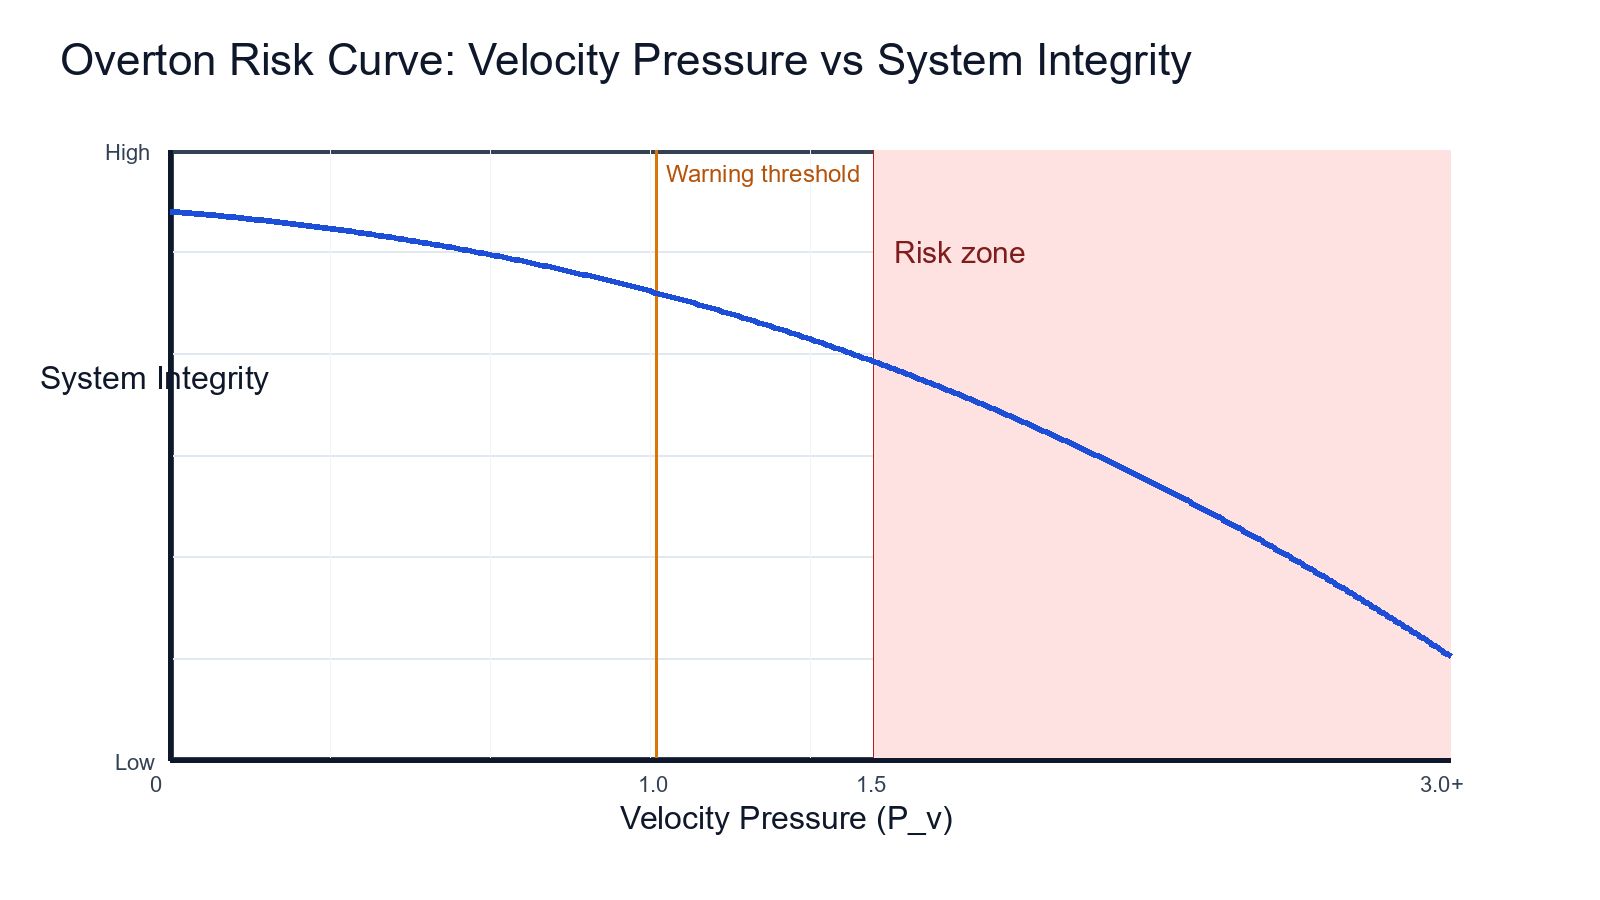
\includegraphics[keepaspectratio,alt={Overton Risk Curve: Velocity Pressure vs System Integrity}]{figures/overton-risk-curve.png}}

As velocity pressure increases, \textbf{system integrity declines}
unless interlocks intervene.

\begin{center}\rule{0.5\linewidth}{0.5pt}\end{center}

\section{12 Empirical Appendix: Velocity Pressure in
Practice}\label{12-empirical-appendix-velocity-pressure-in-practice}

This appendix demonstrates direct operational use of the Velocity
Pressure metric.

\subsection{12.1 Scenario}\label{121-scenario}

Team profile (single working day):

\begin{itemize}
\tightlist
\item
  AI-assisted generation output: 1,200 DBR units/day
\item
  Human verification capacity: 600 DBR units/day
\end{itemize}

Where DBR (Diff-Bounded Review) units represent normalized reviewable
change volume.

\subsection{12.2 Calculation}\label{122-calculation}

Using the framework equation:

\[
P_v = \frac{R_g}{C_v}
\]

Substitution:

\[
P_v = \frac{1200}{600} = 2.0
\]

\subsection{12.3 Interpretation}\label{123-interpretation}

At \(P_v = 2.0\), generation exceeds verification capacity by 100\%.

This places the system in a \textbf{critical cognitive bypass regime}
with a doubling verification backlog per cycle if controls do not
intervene.

\subsection{12.4 Required Control
Response}\label{124-required-control-response}

Minimum response pattern:

\begin{enumerate}
\def\labelenumi{\arabic{enumi}.}
\tightlist
\item
  Enable Soft Interlocks for all high-impact pathways.
\item
  Activate Hard Interlocks on known red-zone patterns (security, data
  integrity, irreversible operations).
\item
  Enforce Verification Gates on merge and deployment surfaces.
\item
  Emit Observability Gate telemetry for audit and trend monitoring.
\end{enumerate}

Operational objective: reduce sustained \(P_v\) toward \(\leq 1.0\)
through either reduced generation rate, increased verification capacity,
or both.

\begin{center}\rule{0.5\linewidth}{0.5pt}\end{center}

\section{13 Governance Model}\label{13-governance-model}

Effective adoption requires governance structures defining acceptable
development practices.

Key elements include:

\begin{itemize}
\tightlist
\item
  verification standards
\item
  review policies
\item
  risk escalation procedures
\item
  compliance auditing
\end{itemize}

Organizations should periodically evaluate \textbf{velocity pressure
metrics} and adjust controls accordingly.

\begin{center}\rule{0.5\linewidth}{0.5pt}\end{center}

\section{14 Limitations}\label{14-limitations}

The framework assumes generation and verification activities can be
measured reliably.

In practice, measuring \textbf{human verification capacity} is difficult
due to:

\begin{itemize}
\tightlist
\item
  code complexity variation
\item
  reviewer expertise differences
\item
  contextual knowledge requirements
\end{itemize}

This limitation is partially mitigated by Hydrostatic Review Protocol
calibration (Section 10.2), but cross-team comparability and
long-horizon stability remain open empirical questions.

\begin{center}\rule{0.5\linewidth}{0.5pt}\end{center}

\section{15 Future Work}\label{15-future-work}

Future research directions include:

\begin{itemize}
\tightlist
\item
  empirical validation of velocity pressure models
\item
  automated verification systems
\item
  adaptive cognitive interlock mechanisms
\item
  large-scale observational studies of AI-assisted development
  environments
\end{itemize}

These investigations will help determine optimal control strategies.

\begin{center}\rule{0.5\linewidth}{0.5pt}\end{center}

\section{16 Conclusion}\label{16-conclusion}

AI-assisted development introduces unprecedented speed into software
creation.

While this acceleration provides clear productivity benefits, it also
introduces \textbf{structural risk} when generation velocity exceeds
human verification capacity.

The Overton Framework provides a systematic approach for managing this
risk.

By introducing \textbf{cognitive interlocks} and monitoring
\textbf{velocity pressure}, organizations can preserve software
integrity while benefiting from AI-assisted productivity gains.

\begin{center}\rule{0.5\linewidth}{0.5pt}\end{center}

\section{Suggested Citation}\label{suggested-citation}

Overton, K. (2026).\\
\textbf{The Overton Framework: Cognitive Interlocks for Integrity in
AI-Assisted Development Systems.}\\
CrisisCore-Systems. Zenodo.

\end{document}
